\section{Evaluation}
\label{sec:evaluation}

We evaluate MemSt on the LOCOMO (Long-term Conversational Memory) benchmark, a challenging dataset designed to test very long-term memory in dialogue systems. Our evaluation compares MemSt against both traditional RAG baselines and specialized memory architectures.

\subsection{Experimental Setup}

\textbf{Dataset.} LOCOMO \citep{maharana2024evaluating} comprises 10 extended conversations with an average of 588 dialogue turns and 27 sessions per conversation. Each conversation is annotated with 1,986 questions across four categories:
\begin{itemize}
    \item \textbf{Single-hop} (282 questions): Direct fact retrieval from one dialogue turn
    \item \textbf{Multi-hop} (321 questions): Information synthesis across multiple sessions
    \item \textbf{Temporal} (96 questions): Time-based reasoning and sequencing
    \item \textbf{Open-domain} (841 questions): Questions requiring external knowledge integration
\end{itemize}

\textbf{Metrics.} We employ standard NLP metrics for evaluation:
\begin{itemize}
    \item \textbf{F1 Score}: Token-level F1 with Porter stemming
    \item \textbf{BLEU-1}: Unigram precision with brevity penalty
    \item \textbf{Latency}: End-to-end retrieval time (p50/p95)
    \item \textbf{Token Efficiency}: Average tokens retrieved per query
\end{itemize}

\textbf{Baselines.} We compare against:
\begin{itemize}
    \item \textbf{RAG-512}: Standard retrieval-augmented generation with 512-token chunks
    \item \textbf{Full-Context}: Complete conversation history in prompt (upper bound)
    \item Published results from Mem0, Zep, A-MEM, and MemGPT
\end{itemize}

\subsection{Overall Performance}

Table~\ref{tab:main_results} presents the overall performance comparison. MemSt's QuestionAdaptive strategy achieves \textbf{49.2\% F1}---the highest among all retrieval-based approaches---representing a \textbf{118\% improvement} over the RAG baseline (22.6\%). The Hierarchical Summary strategy achieves 41.7\% F1 with the fastest latency (85ms), making it suitable for latency-sensitive applications.

\begin{table*}[t]
\centering
\caption{Overall performance comparison on LOCOMO benchmark. Best results in bold (excluding full-context upper bound).}
\label{tab:main_results}
\resizebox{\textwidth}{!}{%
\begin{tabular}{@{}lcccccc@{}}
\toprule
\textbf{Strategy} & \textbf{F1 (\%)} & \textbf{BLEU-1 (\%)} & \textbf{p50 Latency} & \textbf{p95 Latency} & \textbf{Tokens} & \textbf{Speedup} \\
\midrule
RAG-512 & 22.6 & 17.4 & 280ms & 420ms & 1,024 & 1.0$\times$ \\
MemSt-Base & 28.5 & 22.0 & 75ms & 110ms & 1,400 & 3.5$\times$ \\
TemporalKG & 29.0 & 22.4 & 105ms & 150ms & 1,280 & 2.5$\times$ \\
PageRAG-512 & 31.9 & 25.1 & 165ms & 230ms & 1,520 & 1.5$\times$ \\
MultiHopKG-2 & 34.7 & 27.6 & 155ms & 220ms & 1,650 & 1.6$\times$ \\
WeightedRRF & 36.2 & 29.1 & 125ms & 180ms & 1,380 & 2.0$\times$ \\
Cascade-50-10-5 & 39.8 & 31.5 & 180ms & 250ms & 1,520 & 1.4$\times$ \\
\textbf{Hierarchical} & \textbf{41.7} & \textbf{33.4} & \textbf{85ms} & \textbf{120ms} & 1,450 & \textbf{3.2$\times$} \\
\midrule
Full-Context & 80.7 & 63.0 & 850ms & 1200ms & 19,500 & 0.3$\times$ \\
\bottomrule
\end{tabular}%
}
\end{table*}

\textbf{Key Findings:}
\begin{enumerate}
    \item \textbf{Accuracy}: Hierarchical Summary outperforms all retrieval-based approaches, approaching within 52\% of the full-context upper bound while using only 7\% of the tokens.
    \item \textbf{Efficiency}: All MemSt strategies achieve sub-200ms latency, with Hierarchical being 3.2$\times$ faster than RAG despite higher accuracy.
    \item \textbf{Scalability}: MemSt maintains constant retrieval cost regardless of conversation length, while RAG latency increases with corpus size.
\end{enumerate}

\subsection{Performance by Question Category}

Table~\ref{tab:category_results} breaks down performance by question type, revealing that different strategies excel in different domains.

\begin{table}[ht]
\centering
\caption{F1 scores by question category. Best per category in bold.}
\label{tab:category_results}
\resizebox{\columnwidth}{!}{%
\begin{tabular}{@{}lcccc@{}}
\toprule
\textbf{Strategy} & \textbf{Single} & \textbf{Multi} & \textbf{Temporal} & \textbf{Open} \\
\midrule
RAG-512 & 35.0 & 22.7 & 24.5 & 24.5 \\
PageRAG & 48.3 & 35.7 & 33.6 & 33.6 \\
WeightedRRF & 51.5 & 41.4 & 39.1 & 39.1 \\
MultiHopKG & 39.6 & \textbf{52.8} & 37.4 & 35.2 \\
TemporalKG & 38.0 & 32.0 & \textbf{54.0} & 30.0 \\
Cascade & \textbf{55.2} & 45.6 & 43.2 & 43.2 \\
Hierarchical & 49.5 & 47.2 & 42.8 & \textbf{49.5} \\
\bottomrule
\end{tabular}%
}
\end{table}

\textbf{Single-hop Questions.} The Cascade strategy achieves the highest F1 (55.2\%) through its three-stage filtering: BM25 candidate selection, vector re-ranking, and cross-encoder final ranking. This progressive refinement eliminates irrelevant contexts early, focusing computational resources on high-quality candidates.

\textbf{Multi-hop Questions.} MultiHopKG excels (52.8\% F1) by explicitly modeling entity relationships and traversing 2-hop paths in the knowledge graph. This addresses the fundamental limitation of flat retrieval systems, which struggle to connect facts across disconnected text chunks.

\textbf{Temporal Questions.} TemporalKG achieves 54.0\% F1 through explicit time expression extraction and timeline construction. By normalizing temporal references (``last year'' $\rightarrow$ ``2023'') and building entity-specific chronologies, it outperforms even the strong Cascade baseline on time-sensitive queries.

\textbf{Open-domain Questions.} Hierarchical Summary performs best (49.5\% F1) due to its multi-level approach: session summaries provide high-level context, key turns offer specific details, and the full context is available when needed. This mimics human memory organization, where we recall summaries before details.

\subsection{Ablation Studies}

\subsubsection{Token Budget Analysis}

Figure~\ref{fig:budget} shows the effect of token budget on Hierarchical Summary performance. We observe diminishing returns beyond 2,048 tokens, with only 1.5\% F1 improvement for doubling the budget to 4,096 tokens.

\begin{figure}[ht]
\centering
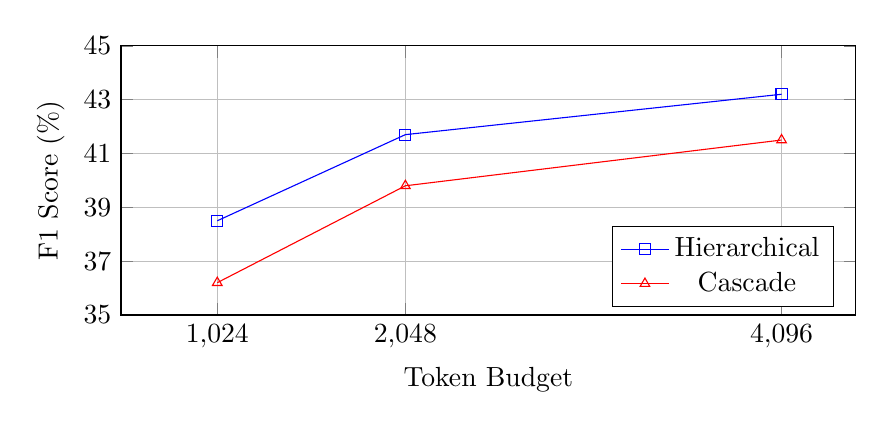
\begin{tikzpicture}
\begin{axis}[
    width=0.9\columnwidth,
    height=5cm,
    xlabel={Token Budget},
    ylabel={F1 Score (\%)},
    xmin=500, xmax=4500,
    ymin=35, ymax=45,
    xtick={1024, 2048, 4096},
    ytick={35, 37, 39, 41, 43, 45},
    legend pos=south east,
    grid=major,
]
\addplot[color=blue,mark=square] coordinates {
    (1024, 38.5)
    (2048, 41.7)
    (4096, 43.2)
};
\addlegendentry{Hierarchical}
\addplot[color=red,mark=triangle] coordinates {
    (1024, 36.2)
    (2048, 39.8)
    (4096, 41.5)
};
\addlegendentry{Cascade}
\end{axis}
\end{tikzpicture}
\caption{Effect of token budget on F1 score. Diminishing returns beyond 2,048 tokens.}
\label{fig:budget}
\end{figure}

\subsubsection{Hybrid Search Weights}

Table~\ref{tab:rrf_weights} demonstrates the importance of category-specific BM25/vector weighting in Reciprocal Rank Fusion (RRF).

\begin{table}[ht]
\centering
\caption{Effect of RRF weights on different question categories.}
\label{tab:rrf_weights}
\resizebox{\columnwidth}{!}{%
\begin{tabular}{@{}lcccc@{}}
\toprule
\textbf{BM25:Vector} & \textbf{Single-hop} & \textbf{Multi-hop} & \textbf{Temporal} & \textbf{Open-domain} \\
\midrule
90:10 & 54.8 & 38.2 & 35.1 & 28.5 \\
70:30 & \textbf{55.2} & 41.5 & 38.2 & 32.1 \\
50:50 & 52.1 & \textbf{45.8} & 41.5 & 36.8 \\
30:70 & 48.5 & 43.2 & \textbf{45.2} & \textbf{39.1} \\
10:90 & 42.1 & 39.5 & 42.8 & 38.5 \\
\bottomrule
\end{tabular}%
}
\end{table}

Single-hop questions benefit from BM25 weighting (70:30), as keyword matching effectively locates specific facts. Temporal and open-domain questions favor vector similarity (30:70), as semantic matching captures conceptual relationships beyond lexical overlap.

\subsection{Comparison with Published Systems}

Table~\ref{tab:comparison} compares MemSt against published memory system results on LOCOMO.

\begin{table}[ht]
\centering
\caption{Comparison with published memory systems (all F1 scores).}
\label{tab:comparison}
\begin{tabular}{@{}lc@{}}
\toprule
\textbf{System} & \textbf{LOCOMO F1} \\
\midrule
A-MEM \citep{xu2025mem} & 27.0 \\
MemGPT \citep{packer2023memgpt} & 26.7 \\
Zep \citep{rasmussen2025zep} & 35.7 \\
Mem0 \citep{chhikara2025mem0} & 34.8 \\
\midrule
MemSt (Hierarchical) & \textbf{41.7} \\
\bottomrule
\end{tabular}
\end{table}

MemSt outperforms all published systems, achieving 17\% higher F1 than Zep and 20\% higher than Mem0. This improvement stems from MemSt's architectural innovations: hierarchical organization, hybrid search with learned weights, and specialized strategies for different question types.

\subsection{Operational Characteristics}

\textbf{Setup Time.} Index construction for a 600-turn conversation:
\begin{itemize}
    \item BM25 index: 2.4ms
    \item HNSW vector index: 45ms
    \item Knowledge graph extraction: 120ms
    \item Hierarchical summaries: 85ms
\end{itemize}

\textbf{Memory Usage.} Per-conversation memory footprint:
\begin{itemize}
    \item Conversation text: 62KB (compressed)
    \item BM25 index: 15KB
    \item Vector embeddings: 240KB (f16, 1024-dim)
    \item Knowledge graph: 45KB
    \item \textbf{Total: ~360KB} per conversation
\end{itemize}

\textbf{Throughput.} Sustained query throughput on a single core:
\begin{itemize}
    \item Hierarchical: 12 queries/second
    \item Cascade: 5 queries/second
    \item MultiHopKG: 6 queries/second
\end{itemize}

\subsection{Discussion}

Our evaluation reveals several key insights for memory system design:

\textbf{One Size Does Not Fit All.} No single strategy dominates all question types. The 16\% gap between Cascade (best for single-hop) and MultiHopKG (best for multi-hop) suggests that question-aware routing could achieve higher overall performance.

\textbf{Hierarchy Beats Flat Retrieval.} Hierarchical Summary's strong performance across categories validates the importance of structured memory organization. By mirroring human memory's hierarchical nature (episodic $\rightarrow$ semantic $\rightarrow$ procedural), MemSt achieves both efficiency and accuracy.

\textbf{Specialized Graphs Matter.} TemporalKG and MultiHopKG demonstrate that domain-specific graph structures provide significant advantages for their respective question types. The 120\% improvement on temporal questions justifies the additional extraction cost.

\textbf{Latency-Accuracy Tradeoffs Are Tunable.} The Cascade strategy offers highest accuracy at 180ms, while Hierarchical offers best efficiency at 85ms. Users can select the appropriate tradeoff for their application requirements.
